\chapter{Metod}
\label{cha:method}
Det här kapitlet går igenom hur arbetet med projektet gick från krav till slutprodukt, vilka ansvarsområden varje medlem hade, vilka resurser användes och hur arbetet dokumenterades. 

\section{Projektstruktur}
I början av kursen så fick alla välja tilltänkta roller som ingår i ett kandidatprojekt i kursen TDDD96 på Linköpings universitet. En projektplan utarbetades som lade grunden för gruppens arbete. Några viktiga riktlinjer och ansvarsområden som har guidat gruppen genom kandidatprojektets gång tas upp här.

\subsection{Gruppens roller}
Projektet strukturerades från början i att alla fick välja tilltänkta roller som togs upp i början av kursen. Följande struktur uppnåddes.

%strukturerad i samma ordning som identiteten
\begin{description}[leftmargin=!,labelwidth=\widthof{\bfseries Konfigurationsansvarig}] %längsta ordet
	\item[Testledare] \textit{Joakim Argillander} - ansvarar för att en testplan finns och följs enligt överenskommen standard, ser till att krav testas och att testfall finns för alla testbara krav.	
	\item[Kvalitetsansvarig] \textit{Victor Bodin} - ansvarar för att samordna kvalitetsbeslut och ansvarar för kvalitetsplanen.
	\item[Utvecklingsledare] \textit{Sebastian Callh} - ansvarar för att organisera utvecklingsarbetet. Agerar Scrum master, tar ansvar för att kompetensen som utvecklingsarbetet kräver finns och undanröjer hinder för att gruppen ska kunna utveckla så effektivt som möjligt.
	\item[Analysansvarig] \textit{Rebecca Lindblom} - ansvarar för kontakt mellan kund och grupp, analyserar kundens behov och ser till att en uppdaterad och relevant kravspecifikation finns.
	\item[Teamledare] \textit{Johan Nåtoft} - ansvarar för att kalla till möten, hålla möten, se till att målen följs i tid.
	\item[Arkitekt] \textit{Johan Thornström} - ansvarar för att ha en översiktlig syn över implementationen och ska kunna fatta beslut om kodens struktur.
	\item[Konfigurationsansvarig] \textit{Jonathan Wahlund} - ansvarar för att versionshanteringen fungerar, hittar lösningar på problem som uppkommer med de verktyg vi använder samt har koll på kod för att kunna ta beslut angående kodpublicering till kund.
	\item[Dokumentansvarig] \textit{Daniel Wassing} - ansvarar för att protokoll förs på möten, ser till att standarder finns och följs för dokument, ser till att det finns ansvariga för alla dokument.
	
\end{description}
En kort riskanalys genomfördes, och det stod klart att det det var en ganska stor risk för projektets genomförande om medlemmar reste bort eller blev sjuka. Därför tilldelades även alla roller en ersättare om huvudansvarig för en viss roll skulle vara otillgänglig av olika anledningar. Denna ersättare byttes ibland ut vid behov då situationen krävde det, men det gav gruppen riktlinjer att jobba efter.

\subsection{Resurser} 
Hela gruppen har haft en tidsbudget på 3200 timmar. Dessa fördelades jämnt på åtta personer, så varje person förväntades arbeta 400 timmar med projektet.
\\ \\
Gruppen hade en handledare att tillgå samt lokaler på Linköpings universitet. Kunden tillhandahöll även en virtuell server för testning under applikationens utveckling.

\subsection{Dokumentation}
Gruppen använde Google Drive för att hantera alla typer av dokument som hade med internt arbete att göra. Bland annat ingick här flera standarder om hur dokument och kod skrevs, hur gruppen konfigurerade Git, hur gruppen använde Trello och diverse installationsguider.
\\ \\
Alla dokument som levererades till kund producerades med hjälp av LaTeX och versionshanterades genom Git.

\begin{table}[h!]
  \centering
  \caption{En tabell över producerade dokument.}
  \def\arraystretch{1.5}
  \begin{adjustbox}{max width=\textwidth}
    \begin{tabularx}{\textwidth}{ | l | X | }
      \hline
      \textbf{Dokument} & \textbf{Beskrivning} \\
      \hline
      Projektplan & Projektets plan över lag, förklarade hur gruppen skulle arbeta \\
      \hline
      Kravspecifikation & Kraven som ställdes på applikationen återges här \\
      \hline
      Kvalitetsplan & Detaljerade beskrivningar om hur arbetet fungerade \\
      \hline
      Arkitekturbeskrivning & Beskrev applikationens struktur \\
      \hline
      Systemanatomi & Visualiserade applikationens anatomi \\
      \hline
      Testplan & Beskrev hur gruppen skulle testa under utvecklingens gång \\
      \hline
      Testrapport & Resultat och utvärdering av hittills utförd testning \\
      \hline
    \end{tabularx}
  \end{adjustbox}
  \label{tab:produced_documents}
\end{table}
\ \\
En lista på producerade dokument återges i tabell \ref{tab:produced_documents}.

\subsection{Möten}
Gruppen hade ett större internt möte varje vecka, vanligtvis måndagar för att samtidigt kunna planera veckan. Utöver interna gruppmöten så hölls handledarmöten nästan varje vecka med gruppens handledare för att få kommentarer på gjort arbete och förslag på kommande arbete.
\\ \\
Kundmöten tog plats under projektets gång, med högre frekvens i början för att hjälpa till med informationsinsamlingen. Bland annat så gavs kommentarer och åsikter på prototypningen av den tänkta slutprodukten.
\\ \\
Både gruppmöten och handledarmöten hade protokoll-skal som användes vid varje möte med en tydlig dagordning för mötet. Dagordningen spikades alltid i början av mötet. Om medlemmar inte kunde närvara fysiskt på mötet men hade tillgång till mobil enhet så bjöds de ibland in över digitalt medium. 

\subsection{Intern kommunikation}
\label{sec:internal_communication}
Textbaserad intern kommunikation skedde över en Slack-kanal \cite{website:slack}. Denna kanal var utrustad med rum för olika delar av projektarbetet samt verktyg för att underlätta beslutstagande och informationsspridning. Kommunikation och statusuppdateringar angående utvecklingsarbetet skedde med hjälp av Trello \cite{website:trello}. Trello användes aktivt i Scrum-processen som kan ses i avsnitt \ref{sec:scrum-work-methodology}.

\begin{figure}[h]
  \centering
  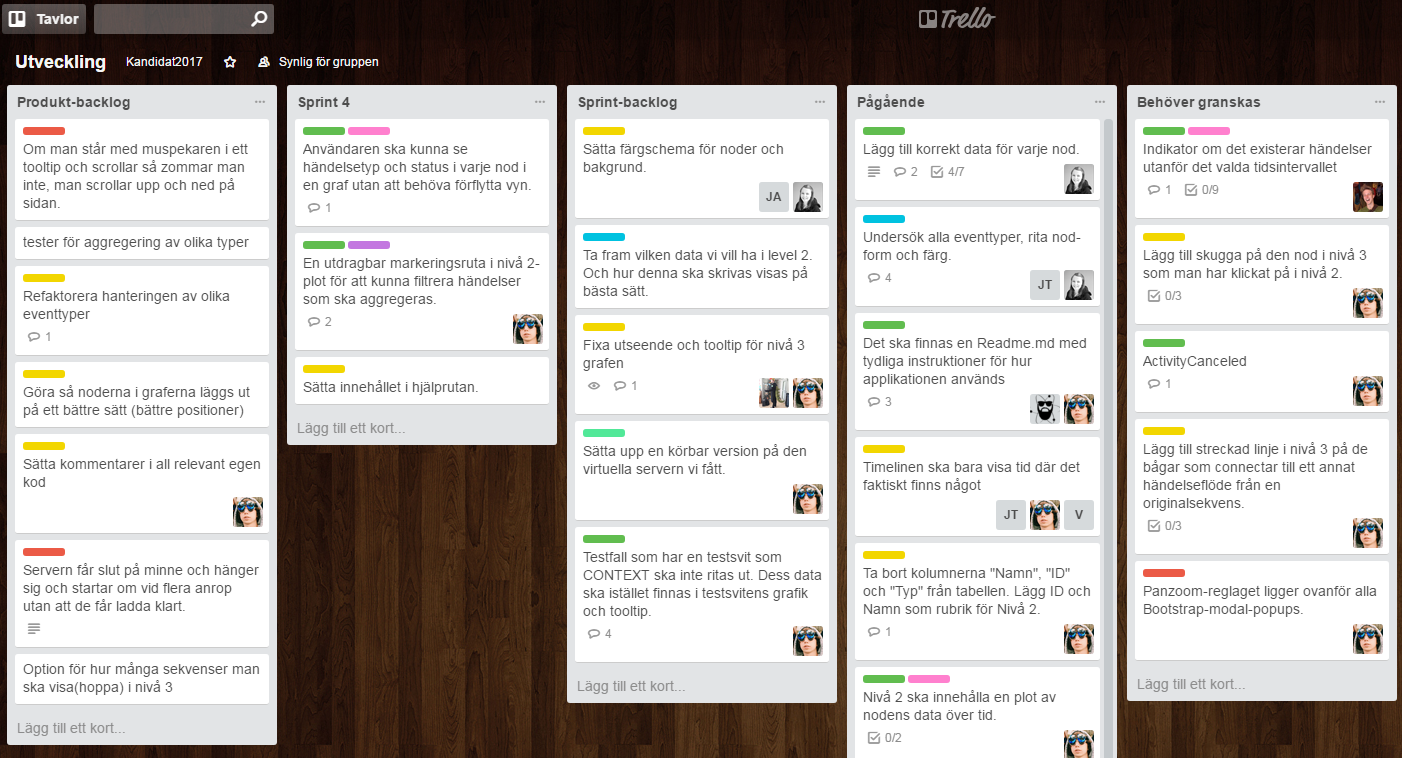
\includegraphics[scale=0.4]{Trello}
  \caption{En illustration över Gruppens arbetsflöde i Trello.}
  \label{fig:trello}
\end{figure}

\subsection{Standarder}
För att säkerställa att allt arbete som gjordes av gruppen skulle hålla en enhetlig standard togs diverse interna standarder fram. De standarder som togs fram var; hur man skriver och ska formulera sig i dokument, vilka stilkonventioner som ska användas vid kodning och för hur testfall för kod ska formuleras.
\\ \\
Förutom enhetlighet i kod, dokument och tester är användning av standarder en viktig del för att säkerställa att det arbete som gjorts av gruppen ska vara lätt att sätta sig in och om vidareutveckling önskas ska inte sättet som dokumentation och utveckling gjorts på vara ett hinder.


\section{Förstudie}
\label{sec:pre-study}
Då både datavisualisering och KI var nytt för hela gruppen spenderades mycket resurser i
början på att förstå projektets direktiv. Ingen konkret tidsplan för studier gjordes dock.
Parallellt så etablerades en projektplan och en kravinsamling påbörjades där en
gränssnittsprototyp användes som hjälpmedel. 
\\ \\
Under förstudien genomfördes en iterativ process kring insamlandet av kraven som kunden ställde på applikationen.
Efter ett flertal kundmöten så kunde gruppen presentera designen av en prototyp som kunden var nöjd med.
\\\\
Då det framgick klart att det var Meteor som skulle användas för appen så sammansattes en presentation om JavaScript som hela gruppen tog del av tillsammans för att få en introduktion till språket. Alla i gruppen installerade den redan befintliga men inte så funktionella prototypen som också den var skriven i JavaScript och Meteor för att få möjligheten att tidigt prova på att utveckla.

\subsection{Kravinsamling}
Gruppens analysansvarig och projektledare intervjuade till en början kunden för att
sammanställa en första kravlista, och fick kort efter kontakt med representanter
för applikationens tänkta slutkunder på företagen Ericsson och Grundfos, som också intervjuades.
\\ \\
Kravinsamlingen har skett i ett flertal iterationer då kraven oftast utvecklades i och med de kundmöten som genomfördes.
Kunden har haft svårt att se varenda aspekt i designen av applikationen från början och det blev naturligt att fler träffar planerades in så att en tillmötesgående design kunde utformas. Vissa krav utvecklades även på grund av problem som stöttes på under utvecklingen.

\subsection{Prototyper}
\label{sec:prototypes}
För att konkretisera och validera de utvunna kraven skapades prototyper. För ett första utkast på prototyp användes 635-metoden \cite{arvolaboken} för att gemensamt i gruppen generera idéer för en första prototyp. Alla i gruppen skapade varsitt förslag för olika delar av gränssnittet, och dessa sammanställdes till en första variant som visades för kund. Efter diskussion med kund och några nya idéer skapades en uppdaterad övergripande version som kom att bli grundstommen för gruppen att arbeta efter. Denna prototyp var dock inte heltäckande för all funktionalitet i systemet. Kravspecifikationen uppdaterades med både förändringar och nya krav för att spegla de mer detaljerade överrenskommelserna med kund. 
\\ \\
Prototypen som i slutändan tagits fram var i pappersform där systemet hade återgetts i de olika nivåerna på separata papper. Vardera pappersprototyp beskrev systemets aktuella nivå på ett rent visuellt sätt så att kunden fick en idé om designens önskvärda målbild. Senare under projeket har även mindre skissliknande pappersprototyper använts internt för att ta fram utseende på mindre delar av applikationen, men alla delar av appliktionen föregicks inte av prototyper. Under projetets gång har de befintliga prototyperna använts som en gemensam designgrund för att utvecklare att utgå från vid utveckling av användargränssnittet.

\section{Utvecklingsmetod}
\label{sec:development-methodology}
Utvecklingen skedde baserat på den agila utvecklingsmetoden Scrum. Eftersom alla gruppmedlemmar inom
projektet hade parallellt pågående kurser och ingen permanent lokal för projektet fanns fick
vissa anpassningar av Scrum göras, som beskrivs nedan. I övriga avseenden användes Scrum som beskrivet
i avsnitt \ref{sec:scrum}.

\subsection{Anpassning av Scrum}
Sprinternas längd valdes till två veckor med motiveringen att gruppen använder Scrum för första gången
och en kortare sprintlängd ger fler möjligheter till anpassning och förbättring vilket förutspåddes
vara behövligt. De dagliga Scrum-mötena som hålls under sprinten bör enligt Scrum hållas vid samma
tid och samma plats varje gång, men då det inte var möjligt p.g.a. gruppmedlemmarnas varierande schema
planerades de veckovis vid tidpunkter där så många som möjligt kunde närvara.
\\ \\
Produktägaren utgjordes av gruppens analysansvarig när det gällde kommunikation med kund. Eftersom
tidigare utbildning inom rollen saknades så beslutades det att analysansvarig inte skulle vara ensam
ansvarig att ta fram projektets produkt-backlog, utan att detta ansvar skulle delas av hela gruppen.
\\ \\
Gruppens Scrum master utgjordes av gruppens utvecklingsledare, som agerade som definierat i Scrum.
Utvecklingsledarens uppgift var främst att organisera scrum-mötena och understödja gruppen
genom att undanröja eventuella hinder för utvecklingen, så som beslut av vilka ramverk och tekniker
som skulle användas eller praktiska frågor om kod.

\subsection{Arbetsflöde}
\label{sec:scrum-work-methodology}
Gruppen arbetade i självorganiserade par. Parprogrammering användes genom hela projektet
eftersom gruppen saknade tidigare erfarenhet med de ramverk och tekniker som användes
och parprogrammering underlättade inlärningen genom att möjliggöra diskussion och att ha
någon att felsöka med. Trello användes för att spåra arbetet och Git användes för att
versionshantera det. I Trello sparades allt arbete som kort i
kolumner “produkt-backlog”, “sprint-backlog”, “pågående”, “behöver granskas” och “klar”.
Projektets Git-användning var strukturerat enligt feature-branch-arbetsflödet. 

\subsubsection{Testning}
Samma personer som skrev ny funktionalitet skrev även testfall för den. Automatiska tester användes
där de kunde men en stor andel av testerna var manuella. För att få sammanfoga
en funktionalitets-gren till utvecklings-grenen behövde ett regressionstest klaras av
tillsammans med de nya testerna.

\subsubsection{Spårbarhet}
För att kunna leverera applikationen mot en kravspecifikation
användes ett system för att spåra krav till färdig implementation.

\begin{figure}[h]
\centering
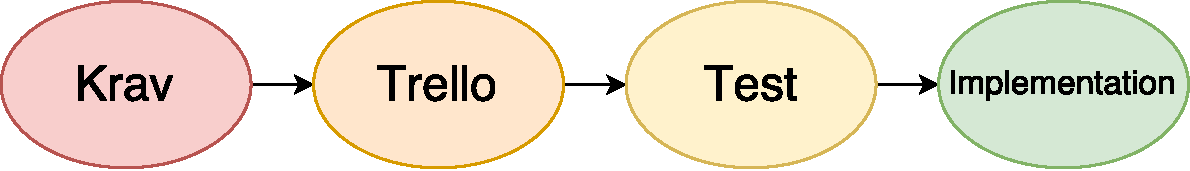
\includegraphics[scale = 0.4]{tracability}
\caption{En illustration över hur spårbarhet uppnåddes.}
\label{fig:tracability}
\end{figure}
\ \\
Krav representerades av Trello-kort, som hade etiketter som visade vilka
krav de kom ifrån. Korten hade även testfall noterade i sina kommentarer, som i sin tur
validerade implementationen. På så sätt var det möjligt att utgåendes från kravspecifikationen se
vilka krav som var mötta genom att notera kravets ID, söka upp korresponderande Trello-kort och utföra
de tester som fanns noterade där. Se figur \ref{fig:tracability} för en illustration över systemet.

\subsection{Arbetsprocess}
Gruppen har från början försökt att hålla sig till sina respektive roller och med minimala rollöverskridanden. Allteftersom projektet har fortskridit har även rollöverskridandet utvecklats. Gruppmedlemmarna har tagit mer ansvar för de olika delarna i arbetet och själva utvecklingsarbetet var även en jämt delad process. Utvecklingen har skett i par om två där samtliga medlemmar har varit involverade på något sätt i att ta fram mjukvara för slutprodukten. Dokumentationen har i största mån skrivits individuellt där gruppmedlemmarna tagit delar de antingen ville skriva om eller var direkt ansvariga för. När en gruppmedlem har upplevt att denna är klar med en del av dokumentationen så tilldelas denna del en form av rättningsansvarig som ansvarar för att läsa igenom det aktuella stycket för att godkänna språk och innehåll.